\section{Combustion} % (fold)
\label{sec:combustion}
%
Combustion is the exothermic chemical reaction of a fuel and an oxidizer into
oxidized products and heat.
%
We will only concern ourselves with the combustion of gases, which is the
most common case used in industrial applications.
%
The oxidizer is usually oxygen, while fuels can range from simple ones such as
hydrogen or methane to complex organic fuels.
%

%
A combustion process is a complex system of elementary chemical reactions
transforming various chemical species into each other while absorbing or
releasing heat.
%
It involves reactants and products but also various intermediate species.
%
These intermediates can be more or less stable and are often radicals with
unpaired electrons.
%
The reaction rate of each elementary reaction in an infinitesimal volume is
dependent on the amounts (\ie{}, mass) of the different chemical species as well
as the current temperature.
%
The composition of chemical species is typically represented via their mass
fractions, \ie{}, the fractions of the total mass of the mixture that is occupied
by each species.
%
This introduces density as an additional variable representing the total mass
per unit volume.
%
Inert gases, which do not participate in the reactions directly can still
influence them by their diluting presence.
%

%
The chemical reactions in a flame are intrinsically linked to the fluid motion
of the gas.
%
As the gas is deformed and transported by the flow, the local concentration and
temperature gradients change, which in turn control the diffusion of chemical
species and heat.
%
Through diffusion, the local mixture and temperature changes, which in turn
influences the reaction rates.
%
As the chemical reactions produce or consume heat, the gas expands or contracts,
which in turn influences the fluid's velocity (the expanded gas has to go
somewhere) and viscosity (molecules that are farther away from each other
interact less).
%
This again influences the mixing and transport of the gas, and so the cycle goes
on.
%

%
Gaseous combustion can be classified by the type of flow and the mixing of
reactants.
%
Is the flow laminar or turbulent, and are fuel and oxidizer premixed or
non-premixed?
%
We will discuss the characteristics of flames in each of these regimes in the
following sections.
%
This discussion is largely based on the book ``Theoretical and Numerical
Combustion'' by Poinsot and Veynante~\cite{Poinsot2012}.
%
\subsection{Laminar Flames} % (fold)
\label{sub:laminar_flames}
%
If the reacting gases in a flame move at low velocities, the flow is often
laminar.
%
Laminar flow is characterized by the absence of eddies or vortices.
%
Layers of the fluid slide past each other without significant mixing.
%
In many cases, the flow is steady in this regime.
%

%
Even though laminar flames are the exception in industrial applications, their
simplicity and deterministic behavior makes them an ideal basis for the
theoretical study of combustion processes.
%
They are the reference case that turbulent combustion is compared against and
that turbulent combustion models are derived from.
%
\subsubsection{Laminar Premixed Flames} % (fold)
\label{ssub:laminar_premixed_flames}
%
In a premixed flame, fuel and oxidizer are brought into a uniform mixture before
ignition.
%
The defining feature of premixed combustion is the flame front that propagates
into the fresh gases and leaves behind hot combustion products.
%
In the simplest case, the flame front is planar and travels along its normal
direction.
%
In this case, the phenomenon is essentially one-dimensional (see
\cref{fig:premixed_profiles}).
%
\begin{figure}[t]
    \centering
    % \MissingFigure{\ac{1D} profiles of an ideal premixed flame}
    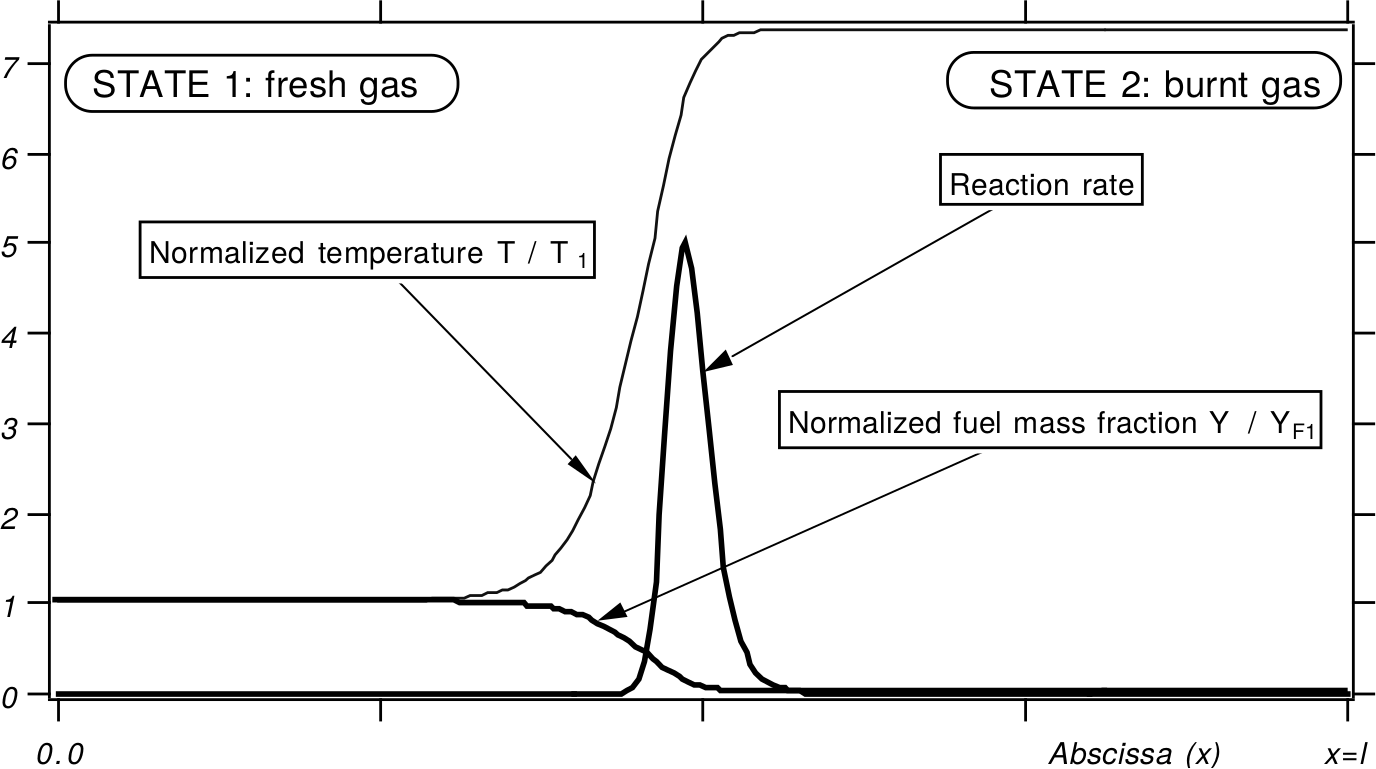
\includegraphics[width=\textwidth]{figures/1D_premixed_flame.png}
    \caption{Basic configuration of a one-dimensional laminar premixed flame.
    Image source: Poinsot and Veynante~\cite{Poinsot2012}}
    \label{fig:premixed_profiles}
\end{figure}
%
The profiles of the combustion variables along the normal direction show high
concentrations of fuel and oxidizer on the fresh gas side and high combustion
product concentrations and temperature on the burnt gas side.
%
In between the two extrema is the flame front that shows the gradual transition
between fresh and burnt gases.
%
The concentration of intermediate species is highest in the flame front.
%
Intermediates generally do not occur in the fresh gases, but some radicals may
exist on the burnt gas side due to dissociation of combustion products at high
temperatures.
%
\begin{figure}[tp]
    \centering
    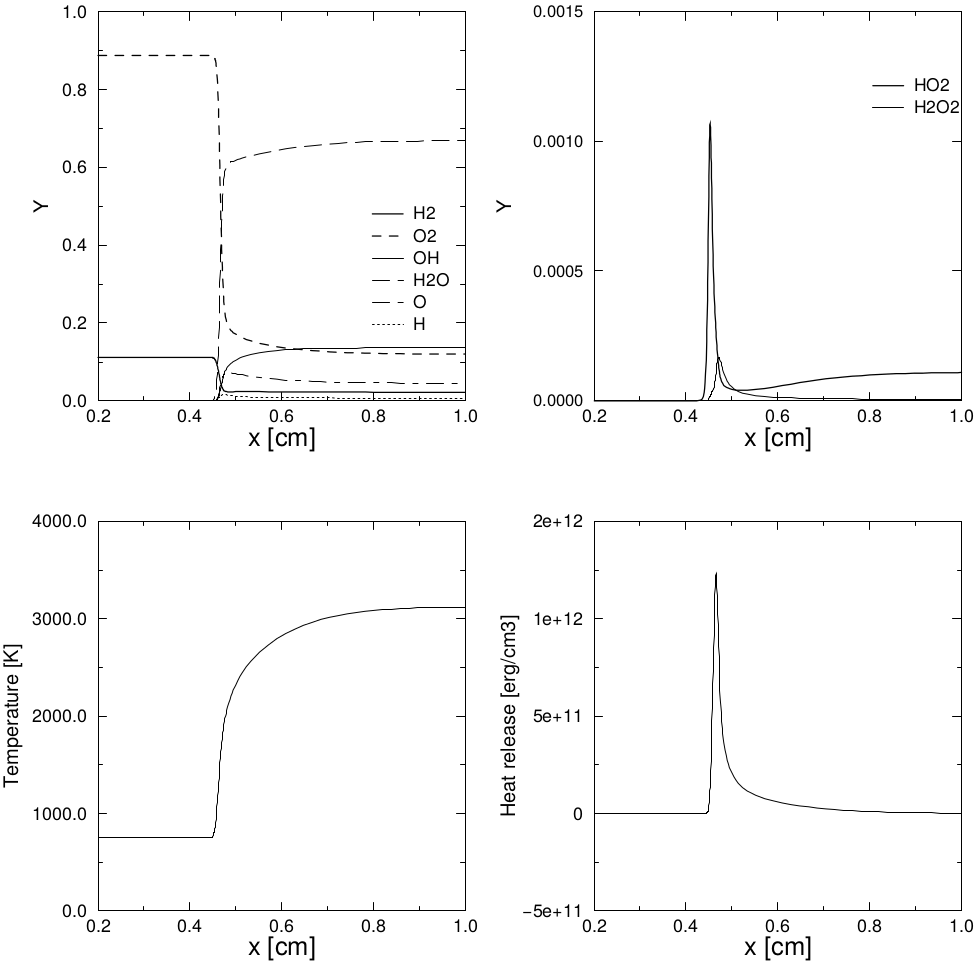
\includegraphics[width=\textwidth]{figures/laminar_flame.png}
    \caption{Profiles of species (Y), temperature and heat release of a
    laminar premixed \ce{H2}-\ce{O2} flame. Image source: Poinsot and
    Veynante~\cite{Poinsot2012}}
    \label{fig:laminar_premixed_profiles}
\end{figure}

%
The characteristic properties of a premixed flame front are \emph{flame speed},
\emph{flame stretch}, and \emph{flame thickness}.
%
These three quantities depend on each other and the underlying flow field.
%

%
The flame speed is the speed at which the flame front travels.
%
It can be expressed relative to a laboratory frame of reference, or relative to
the flow.
%
Sometimes, it is also expressed as the speed at which fresh gases are turned
into combustion products.
%
The flame speed can vary considerably along the surface of a flame, and
depending on conditions, the flame front can travel against the flow at
considerable speeds.
%

%
The flame thickness describes the width of the reaction zone normal to the flame
front.
%
Depending on the application, it is determined in different ways.
%
One common definition uses the slope at the point of highest temperature
gradient.
%
Another one is based on the distance between the isosurfaces of minimum and
maximum temperature.
%
Different alternative definitions exist as well, some of them based on radical
species.
%
The flame thickness is inversely proportional to the flame speed in canonical
configurations.
%
A thinner flame travels more quickly and slow-moving flames tend to be thicker.
%
Flame thickness is an essential measurement for combustion simulations, as it
determines the grid resolution necessary to resolve the flame front.
%

%
Both flame speed and flame thickness are dependent on the chemical reaction
taking place and the stretch of the flame front.
%
Flame stretch is the change in surface area an infinitesimal element of the
(idealized) flame surface experiences over an infinitesimal time interval.
%
It can be induced by a non-uniform flow, but also by the expansion or
contraction a curved flame front experiences due to its propagation in normal
direction.
%
\Cref{fig:stretched_premixed_flames} shows some examples of stretched laminar
premixed flames.
%
If the flame experiences positive stretch, it is tangentially expanded and
compressed in normal direction.
%
This decreases the flame thickness and feeds new fresh gases to the reaction,
which increases the flame speed.
%
However, it also increases heat dissipation.
%
If the flame is stretched too quickly, this can lead to quenching.
%
Negative stretch (compression) leads to less fresh gas being transported near
the reaction zone, which increases the flame thickness and reduces flame speed.
%
\begin{figure}[tp]
    \centering
    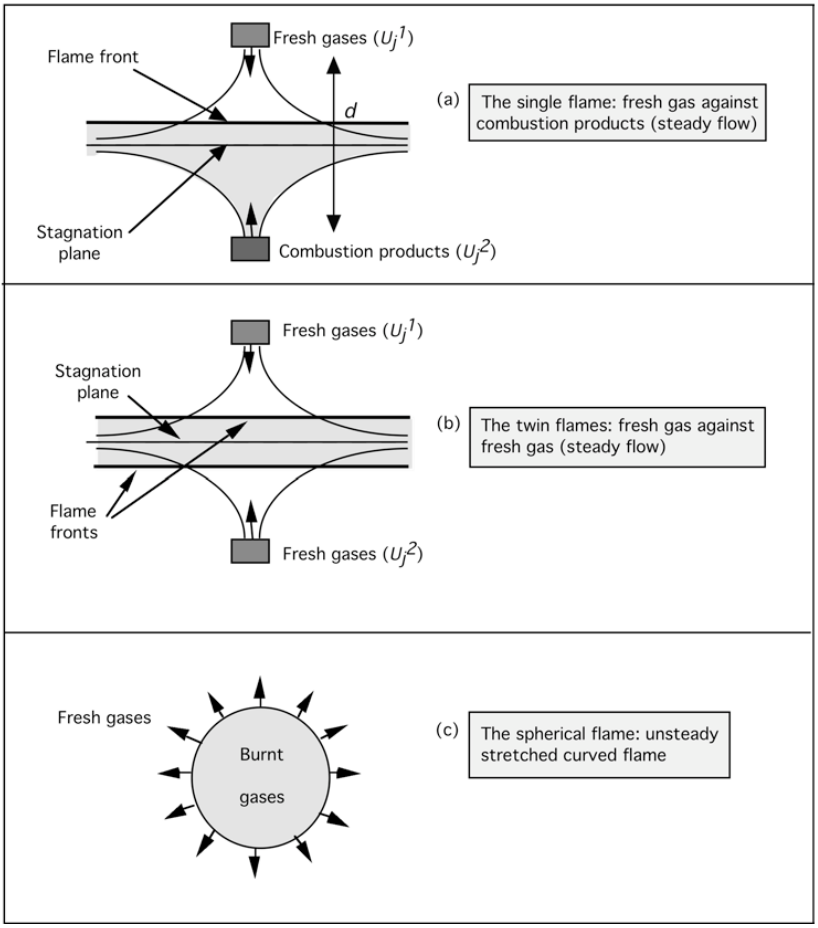
\includegraphics[width=\textwidth]{figures/stretched_premixed_flames.png}
    \caption{Examples of stretched laminar premixed flames. Image source:
    Poinsot and Veynante~\cite{Poinsot2012}}
    \label{fig:stretched_premixed_flames}
\end{figure}

%
Due to their defining characteristic for the behavior of the flame, flame speed,
thickness and stretch are the basis for a lot of combustion models, and a focus
of study in many combustion experiments and simulations.
%
% subsubsection laminar_premixed_flames (end)
%
\subsubsection{Laminar Non-Premixed (Diffusion) Flames} % (fold)
\label{ssub:laminar_diffusion_flames}
%
In non-premixed combustion, fuel and oxidizer are supplied separately.
%
Combustion can only occur where both mix in a sufficient ratio via diffusion.
%
This is why non-premixed flames are also called diffusion flames.
%
\Cref{fig:laminar_diffusion_profiles} shows a \ac{1D} cross-section of a
typical laminar diffusion flame.
%
\begin{figure}[t]
    \centering
    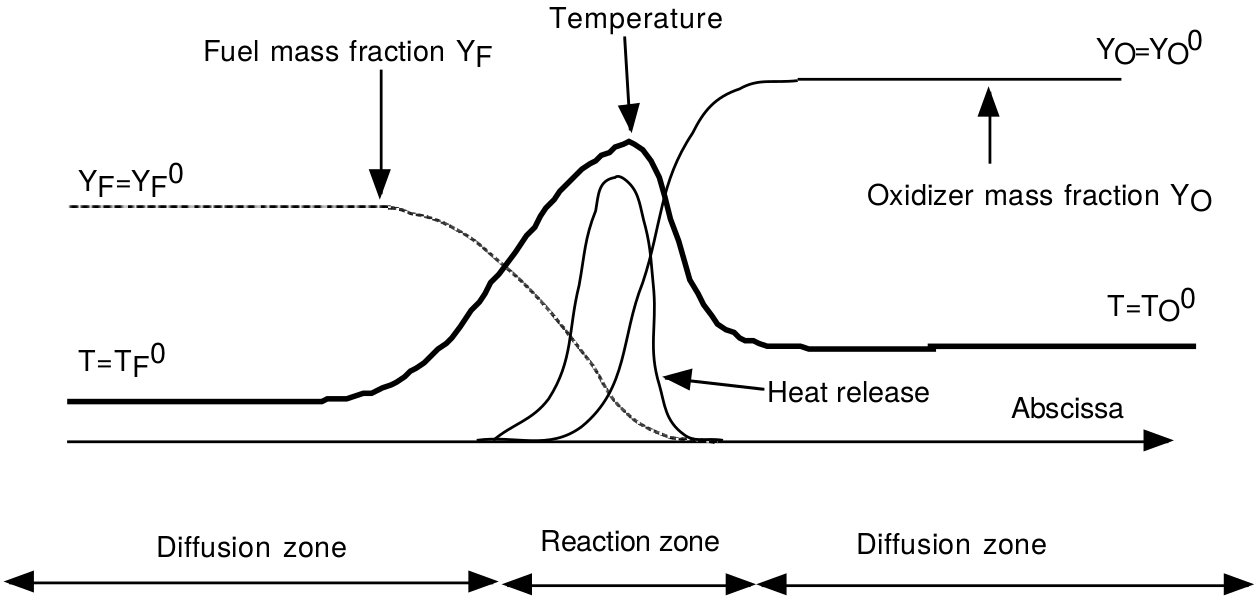
\includegraphics[width=0.8\textwidth]{figures/laminar_diffusion_flame.png}
    \caption{Basic configuration of a one-dimensional laminar diffusion flame.
    Image source: Poinsot and Veynante~\cite{Poinsot2012}}
    \label{fig:laminar_diffusion_profiles}
\end{figure}
%

%
The prototypical example of a diffusion flame is a jet flame where fuel gas is
injected into ambient air and ignited.
%
An example of this type we are all familiar with is the flame of a candle.
%
Wax is evaporated from the wick via the heat of the flame.
%
This fuel gas burns as it comes into contact with ambient air and creates a
laminar diffusion flame.
%
The heat generated from the flame is sufficient to ignite the fresh fuel being
supplied from the wick and sustain the reaction.
%
\Cref{fig:laminar_diffusion_jet} shows a simplified example of such a flame.
%
\begin{figure}[t]
    \centering
    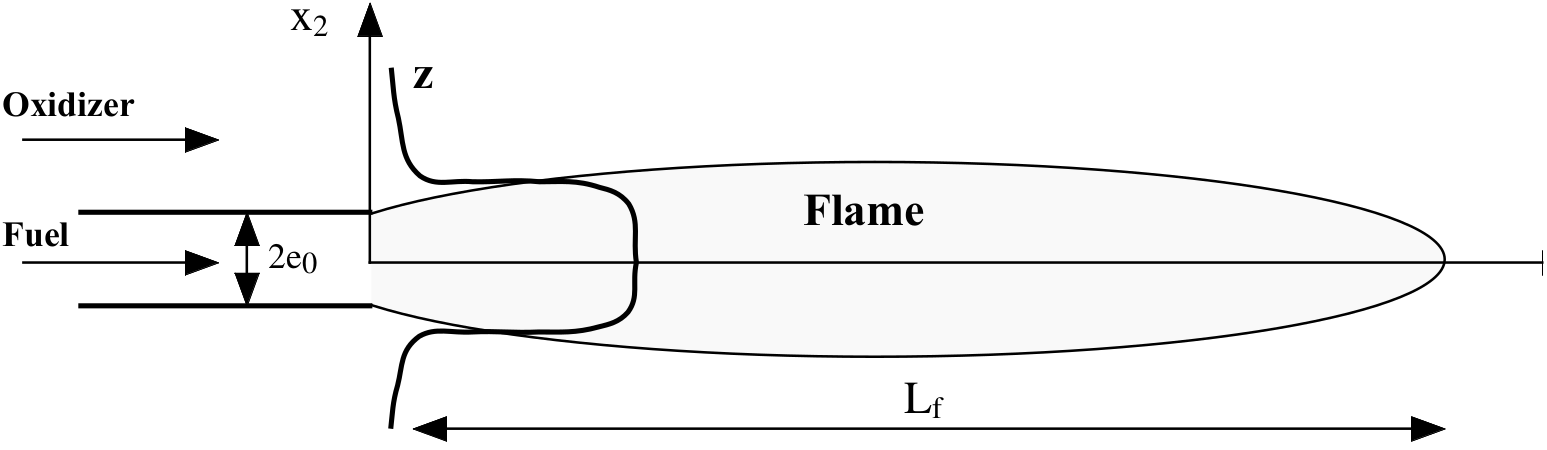
\includegraphics[width=0.8\textwidth]{figures/laminar_diffusion_jet.png}
    \caption{Simple \ac{2D} laminar diffusion jet flame. Image source: Poinsot
    and Veynante~\cite{Poinsot2012}}
    \label{fig:laminar_diffusion_jet}
\end{figure}
%

%
Diffusion flames are easier to set up than premixed flames from a practical
perspective, as no perfect mixing of fuel and oxidizer is required beforehand.
%
They are also safer because they prevent flashbacks into the gas supply.
%
However, it is harder to ensure a clean and complete consumption of fuel in
non-premixed combustion.
%
This is why diffusion flames are generally less efficient and produce more
soot and pollutants that result from suboptimal burning conditions.
%

%
As the conditions for combustion are not satisfied initially, transport and
mixing become the main issues in a non-premixed flame.
%
Fuel and oxidizer need to mix sufficiently to create a combustible mixture.
%
Temperature produced by nearby combustion needs to be high enough to ignite
the mixture.
%
Combustion products need to be transported away from the combustion zone fast
enough to prevent the flame from suffocating, but not too fast to dissipate the
heat required for continued combustion.
%

%
Diffusion flames do not propagate like premixed flames.
%
Their position is fixed at the interface between fuel and oxidizer.
%
For this reason, the speed of the flame is not a relevant quantity for
analyzing the behavior of diffusion flames.
%
Instead, the defining variable is the mixture fraction between fuel and
oxidizer.
%
The flame is generally strongest where the mixture fraction is near
stoichiometry, \ie{}, where fuel and oxidizer are mixed in such a ratio that
both are consumed completely by the reaction.
%
Mixture fraction and temperature are the dominating variables controlling a
diffusion flame, which is why simple combustion models are based on these two
quantities.
%

%
Unlike for premixed flames, where it mainly influences the speed of the reaction
and can only quench the flame in extreme cases, diffusion flames are very
sensitive to flame stretch.
%
A certain stretch is necessary to supply fresh gases to the reaction zone and
transport away combustion products that would otherwise suffocate the flame.
%
However, for high flame stretch heat might be dissipated too quickly to sustain
the reaction, leading to extinction.
%

%
Because diffusion flames are much more sensitive to the flow conditions, and
combustion occurs over a wider range of fuel/oxidizer mixture fractions,
modeling and simulating diffusion flames is more challenging than premixed
flames.
%
% subsubsection laminar_diffusion_flames (end)
%
% subsection laminar_flames (end)
%
\subsection{Turbulent Flames} % (fold)
\label{sub:turbulent_flames}
%
Although laminar flames are the basis for the study of combustion, most
industrial combustion applications are turbulent in nature.
%
This makes turbulent combustion an important area of research.
%
Unfortunately, it is also a particularly challenging one.
%
Turbulent flow itself is still not well understood by the scientific community,
and understanding and modeling complex chemical reactions still poses a
significant challenge.
%
In turbulent combustion, both of these phenomena are combined and interact with
each other, which makes understanding even more difficult.
%

%
Turbulent flow is a chaotic and essentially statistical process.
%
It occurs when the inertial force of the flow is dominant over the damping
effect caused by the fluid's viscosity.
%
This happens at higher fluid velocities, where small imperfections lead to
disturbances that are not immediately absorbed by viscous effects.
%

%
Turbulent flow is characterized by a mixture of \emph{eddies} of different sizes
and energies.
%
The sizes of eddies in a flow range from the integral length scale, that is
roughly equivalent to the size of the domain the flow resides in, to the
Kolmogorov length scale, that describes the smallest eddies in the system.
%
The energy in a turbulent flow passes along the turbulent spectrum from the
largest length scales to the smallest ones.
%
Large eddies spin off smaller eddies, which spin off even smaller eddies and so
on until the energy is dissipated as heat at the Kolmogorov scale.
%
This is why turbulent flow will decay over time if it is not continuously
supplied with energy.
%

%
The interaction between flow and chemistry in a turbulent flame is a two-way
street.
%
The reaction transforms and heats the gas, changing its density and viscosity
and thereby influencing the flow.
%
On the other hand turbulent flow transports and mixes the gases, thereby
influencing the conditions for combustion.
%
\begin{figure}[t]
    \centering
    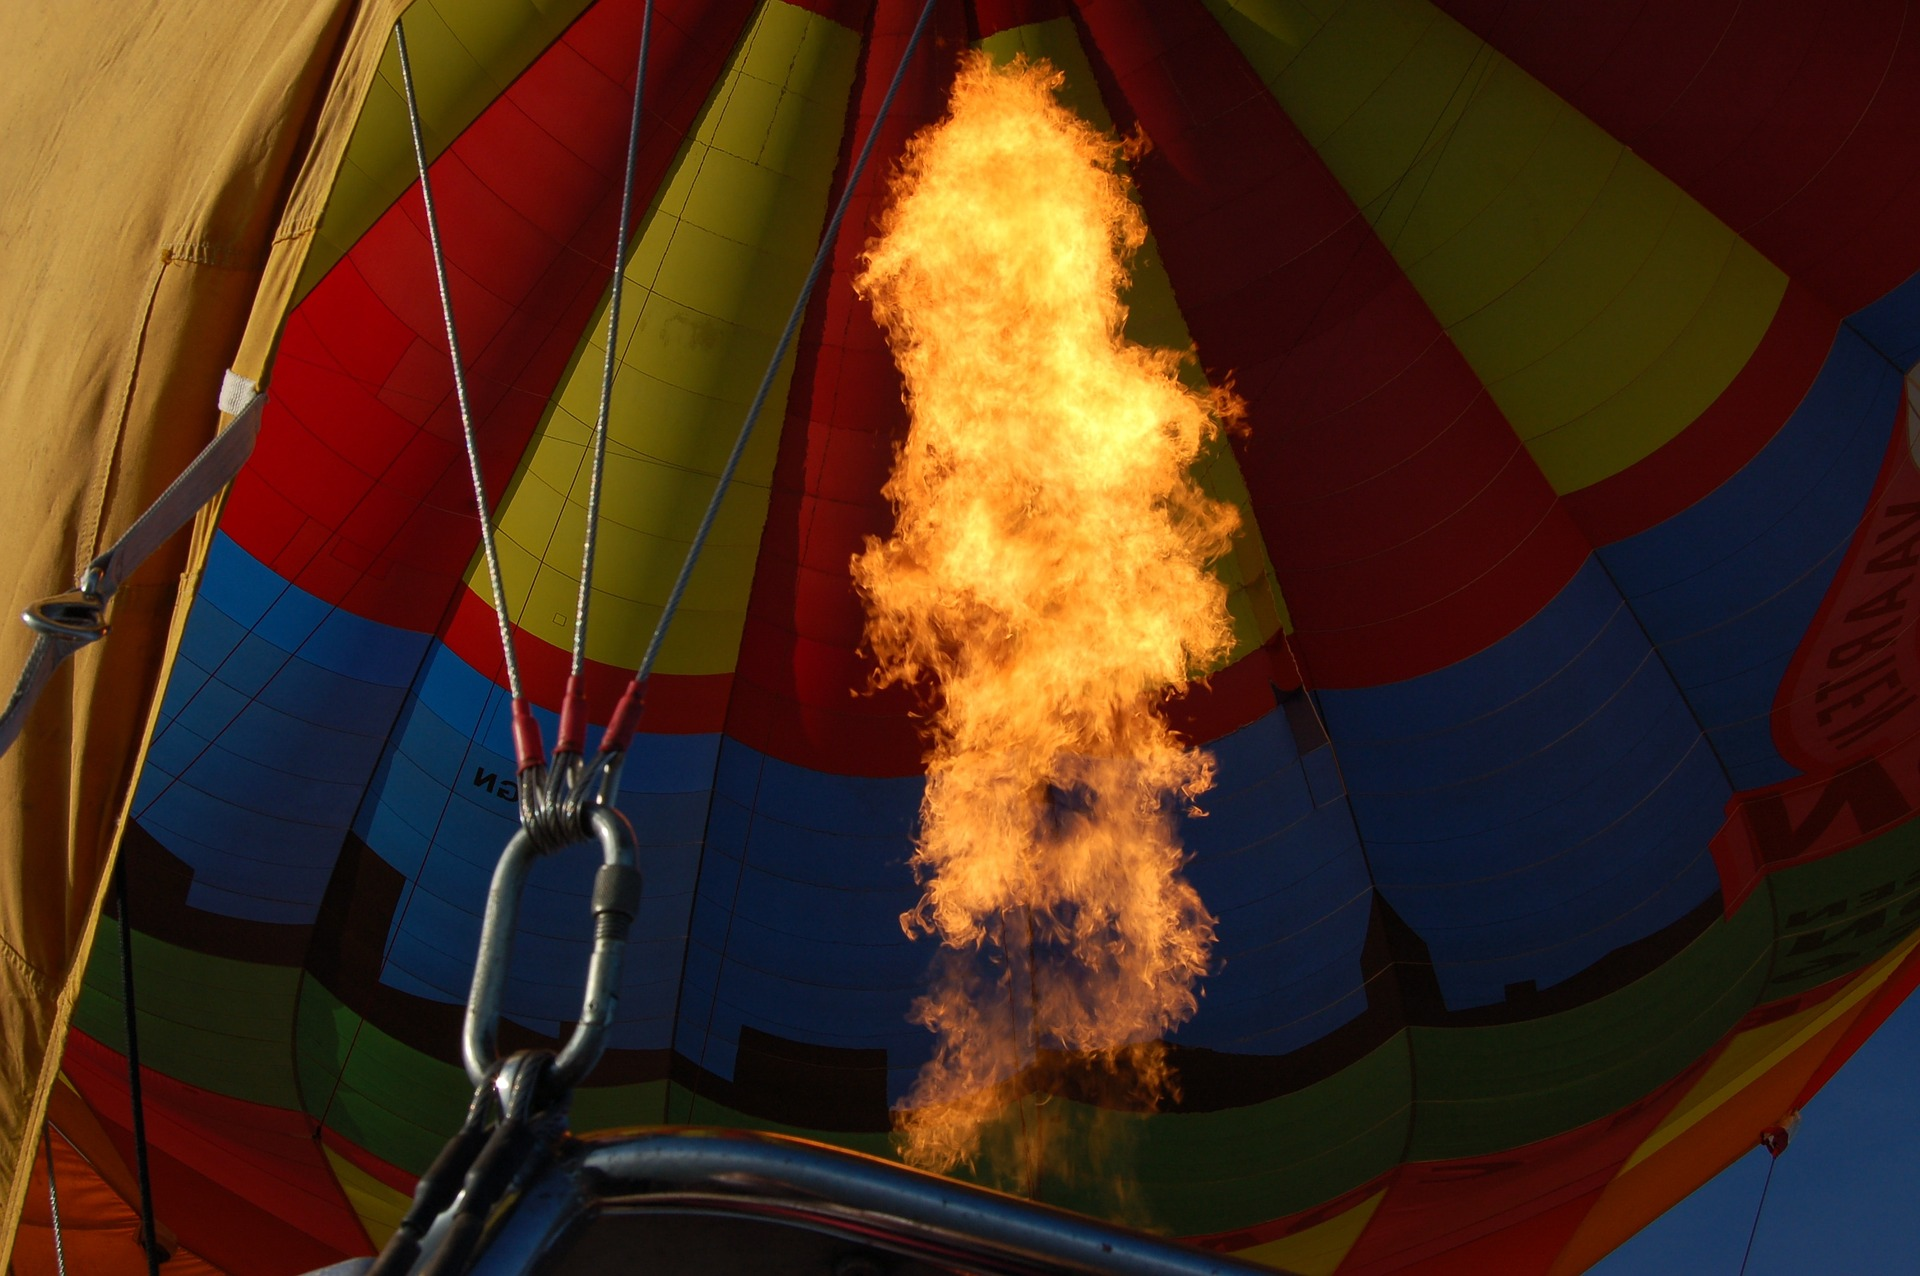
\includegraphics[width=\textwidth]{figures/balloon_burner.jpg}
    \caption{Example of a turbulent non-premixed flame: The burner of a hot air
    balloon.}
    \label{fig:balloon_burner}
\end{figure}
%

%
The effect of turbulence on the flame depends on the size and strength of
the eddies comprising the flow.
%
Large eddies move slowly and only wrinkle the surface in large scales.
%
This only has an indirect effect on the structure of the flame and the chemical
reactions, but influences the global flame shape.
%
Smaller eddies are faster and might disturb the structure of the flame locally.
%
This might have the effect of destroying a clean flame front and causing local
extinction, or it might enhance local mixing and improve the conditions for
combustion.
%
If the eddies are too small, they might be dissipated before they are able to
influence the reaction significantly.
%
Which scales interact with the flame in which way is also dependent on the speed
at which the chemical reaction happens, the flame thickness, and in the case of
premixed combustion, the flame speed.
%
Building accurate models for turbulent combustion requires in\-ves\-ti\-ga\-ting
the interplay of all these variables and more.
%
\subsubsection{Turbulent Premixed Flames} % (fold)
\label{ssub:turbulent_premixed_flames}
%
In premixed flames, turbulence has the primary effect of enhancing combustion.
%
The turbulent flow wrinkles the flame surface and increases its surface area.
%
A higher surface area means that reaction happens at more places at once.
%
The global flame speed increases and fresh gases are consumed more rapidly.
%
However, at high turbulence intensities, the heat produced by the reaction
will be dissipated too quickly and the flame might be extinguished.
%

%
Due to the massive change in viscosity on the burnt gas side, the turbulence
intensity in premixed flames is typically much stronger in the fresh gases.
%
This difference is so significant that the flow on the burnt gas side may become
laminarized, depending on the initial turbulence intensity.
%

%
In practice, premixed combustion occurs for example in spark-ignited internal
combustion engines.
%
Here, air-fuel mixture is sucked into the cylinder, compressed and then ignited.
%
Starting from the ignition point, the flame front travels through the cylinder,
being wrinkled by the turbulent flow of the gas and transforming fresh gases
into hot combustion products.
%
% subsubsection turbulent_premixed_flames (end)
%
\subsubsection{Turbulent Diffusion Flames} % (fold)
\label{ssub:turbulent_diffusion_flames}
%
The typical diffusion flame setup is the jet flame.
%
A stream of fuel gas, often turbulent, is injected into ambient air.
%
Mixing between fuel and air is provided by the turbulent shear layer that arises
from the difference in velocities between the two gases.
%
This leads to a reaction zone that is typically very thin at the outlet and
becomes thicker as more mixing occurs downstream, where a substantial volume is
occupied by combustion products.
%
A practical example for a diffusion jet flame is shown in
\cref{fig:balloon_burner}.
%

%
A central problem of turbulent diffusion flames is flame stabilization.
%
Typically, combustion does not start directly after the fuel gas leaves the
inlet, but only after some mixing has occurred.
%
This mixed gas then needs to be ignited by already-burning mixture further
downstream.
%
This lateral propagation of the flame needs to happen at least at the same
velocity as the flow, otherwise the flame will be blown off.
%
To make this process more stable, some setups provide small premixed pilot
flames between fuel an air stream to provide a steady source of heat.
%

%
If mixing occurs faster than combustion, or if the flame is locally extinguished
due to high flame stretch, pockets of premixed gas can form that are later
ignited when coming into contact with high-temperature regions.
%
This means that parts of a diffusion flame might actually be in the premixed
regime.
%
This highlights the complexity of diffusion flames compared to premixed flames.
%
Due to the additional problem of mixing, diffusion flames are much more
sensitive to turbulence.
%
Depending on their setup, many different conditions and mechanisms can be in
effect at the same time.
%
This makes non-premixed flames very challenging to model and simulate.
%
% subsubsection turbulent_diffusion_flames (end)
%
% subsection turbulent_combustion (end)
%
% section combustion (end)